\documentclass[letter,12pt,english]{article}

\usepackage[utf8]{inputenc}
\usepackage{pgfplots}
\usepackage{xintexpr}
\pgfplotsset{compat=newest}
\usepgfplotslibrary{groupplots}

\usepackage[margin=1in, showframe]{geometry}
\usepackage{microtype}

\newlength\figureheight
\newlength\figurewidth
\setlength\figureheight{5in}
\setlength\figurewidth{6in}

\begin{document}
\begin{figure}
\centering
% This file was created by matplotlib2tikz v0.7.3.
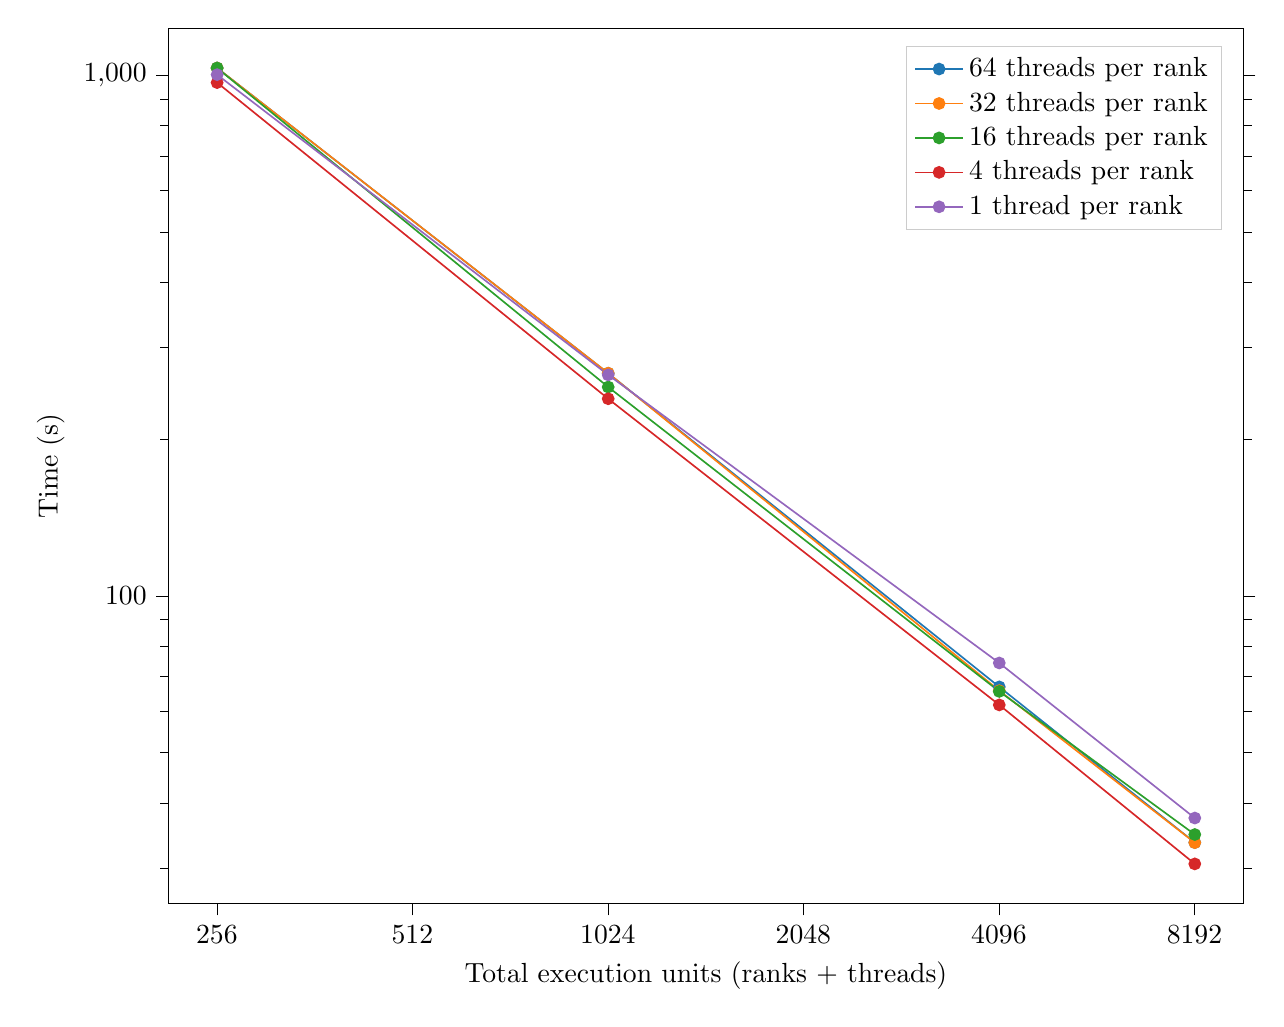
\begin{tikzpicture}

\definecolor{color0}{rgb}{0.12156862745098,0.466666666666667,0.705882352941177}
\definecolor{color1}{rgb}{1,0.498039215686275,0.0549019607843137}
\definecolor{color2}{rgb}{0.172549019607843,0.627450980392157,0.172549019607843}
\definecolor{color3}{rgb}{0.83921568627451,0.152941176470588,0.156862745098039}
\definecolor{color4}{rgb}{0.580392156862745,0.403921568627451,0.741176470588235}

\begin{axis}[
every y tick label/.style = {
rotate=0.0
},
height=\figureheight,
legend cell align={left},
legend style={draw=white!80.0!black},
log basis x={2},
log basis y={10},
log ticks with fixed point,
tick align=outside,
width=\figurewidth,
x grid style={white!69.01960784313725!black},
xlabel={Total execution units (ranks + threads)},
xmin=215.269482304951, xmax=9741.98468610229,
xmode=log,
xtick pos=left,
xtick style={color=black},
xticklabel={\xinttheiexpr[0]2^\tick\relax},
y grid style={white!69.01960784313725!black},
ylabel={Time (s)},
ymin=25.6229808875648, ymax=1231.62057687985,
ymode=log,
ytick pos=both,
ytick style={color=black}
]
\addplot [semithick, color0, mark=*, mark size=2, mark options={solid}]
table {%
8192 33.58101
4096 66.852355
1024 267.678399
256 1032.831161
};
\addlegendentry{64 threads per rank}
\addplot [semithick, color1, mark=*, mark size=2, mark options={solid}]
table {%
8192 33.567934
4096 65.748863
1024 267.762241
256 1032.791601
};
\addlegendentry{32 threads per rank}
\addplot [semithick, color2, mark=*, mark size=2, mark options={solid}]
table {%
8192 34.79345
4096 65.524512
1024 251.86032
256 1032.547306
};
\addlegendentry{16 threads per rank}
\addplot [semithick, color3, mark=*, mark size=2, mark options={solid}]
table {%
8192 30.554646
4096 61.728044
1024 239.114811
256 968.240309
};
\addlegendentry{4 threads per rank}
\addplot [semithick, color4, mark=*, mark size=2, mark options={solid}]
table {%
8192 37.42741
4096 74.320769
1024 265.778503
256 1002.823942
};
\addlegendentry{1 thread per rank}
\end{axis}

\end{tikzpicture}
\caption{Runtime comparison}
\label{fig:runtime-comparison}
\end{figure}

\begin{figure}
\centering
% This file was created by matplotlib2tikz v0.7.3.
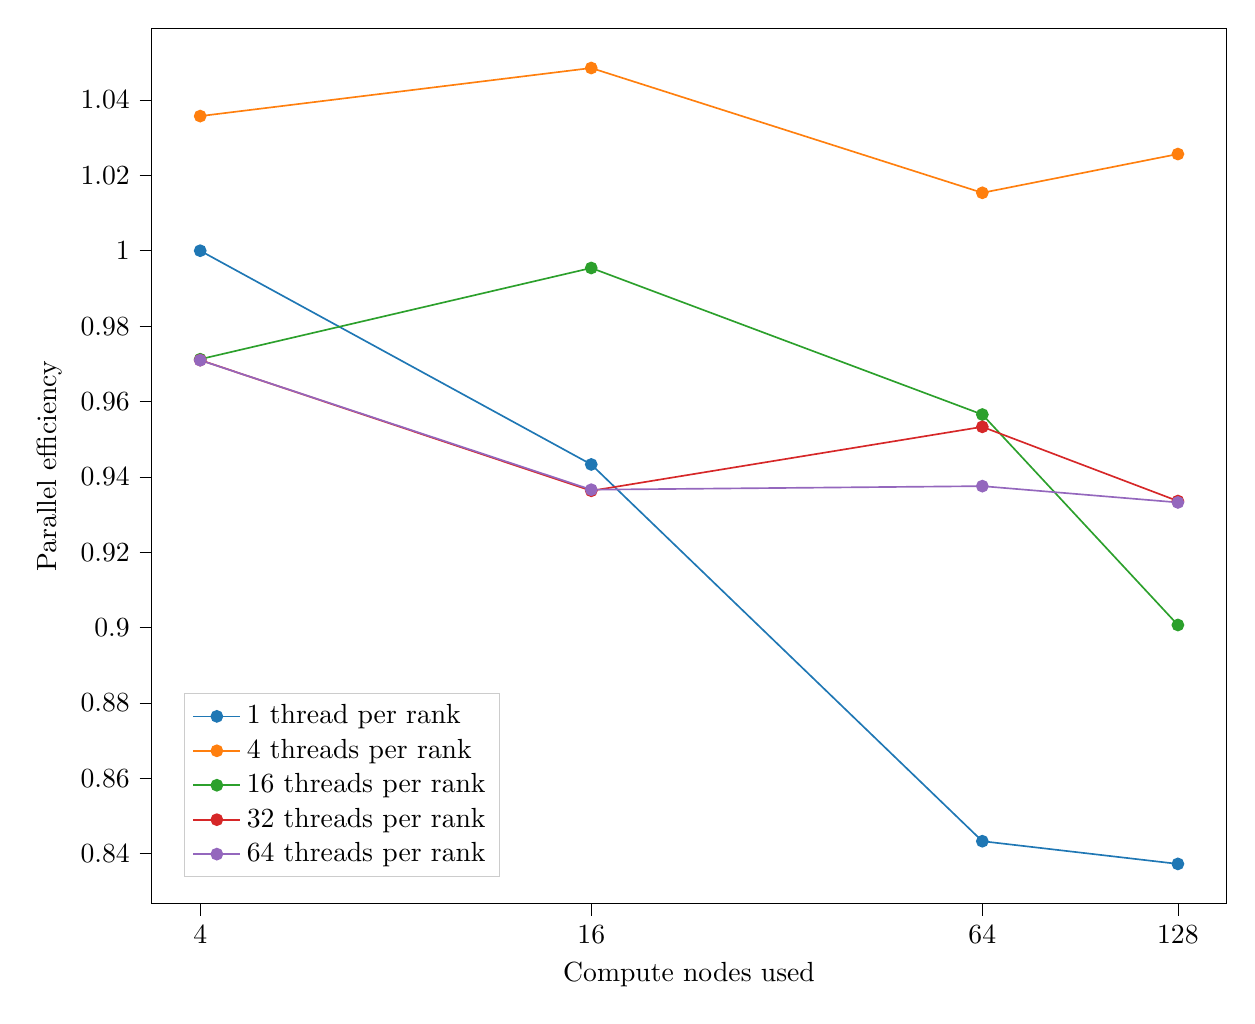
\begin{tikzpicture}

\definecolor{color0}{rgb}{0.12156862745098,0.466666666666667,0.705882352941177}
\definecolor{color1}{rgb}{1,0.498039215686275,0.0549019607843137}
\definecolor{color2}{rgb}{0.172549019607843,0.627450980392157,0.172549019607843}
\definecolor{color3}{rgb}{0.83921568627451,0.152941176470588,0.156862745098039}
\definecolor{color4}{rgb}{0.580392156862745,0.403921568627451,0.741176470588235}

\begin{axis}[
height=\figureheight,
legend cell align={left},
legend style={at={(0.03,0.03)}, anchor=south west, draw=white!80.0!black},
log basis x={2},
tick align=outside,
tick pos=left,
width=\figurewidth,
x grid style={white!69.01960784313725!black},
xlabel={Compute nodes used},
xmin=3.36358566101486, xmax=152.218510720348,
xmode=log,
xtick style={color=black},
xtick={128, 64, 4, 16},
xticklabel={\xinttheiexpr[0]2^\tick\relax},
y grid style={white!69.01960784313725!black},
ylabel={Parallel efficiency},
ymin=0.826749025759338, ymax=1.05903374791091,
ytick style={color=black}
]
\addplot [semithick, color0, mark=*, mark size=2, mark options={solid}]
table {%
128 0.837307422220773
64 0.843324110047893
16 0.943289177529907
4 1
};
\addlegendentry{1 thread per rank}
\addplot [semithick, color1, mark=*, mark size=2, mark options={solid}]
table {%
128 1.02564592590927
64 1.01536501585892
16 1.04847535144948
4 1.03571802648427
};
\addlegendentry{4 threads per rank}
\addplot [semithick, color2, mark=*, mark size=2, mark options={solid}]
table {%
128 0.900693900360556
64 0.956535111242034
16 0.995416767119171
4 0.971213557163646
};
\addlegendentry{16 threads per rank}
\addplot [semithick, color3, mark=*, mark size=2, mark options={solid}]
table {%
128 0.933576912642285
64 0.953271182423337
16 0.936300744136661
4 0.970983827743193
};
\addlegendentry{32 threads per rank}
\addplot [semithick, color4, mark=*, mark size=2, mark options={solid}]
table {%
128 0.933213390172005
64 0.937536102879248
16 0.936594011457757
4 0.970946636649744
};
\addlegendentry{64 threads per rank}
\end{axis}

\end{tikzpicture}
\caption{Parallel efficiency comparison}
\label{fig:efficiency-comparison}
\end{figure}

\begin{figure}
\centering
% This file was created by matplotlib2tikz v0.7.3.
\begin{tikzpicture}

\definecolor{color0}{rgb}{0.12156862745098,0.466666666666667,0.705882352941177}

\begin{axis}[
height=\figureheight,
log basis x={2},
tick align=outside,
tick pos=left,
width=\figurewidth,
x grid style={white!69.01960784313725!black},
xlabel={MPI ranks},
xmin=103.968306733598, xmax=10085.5350341216,
xmode=log,
xtick style={color=black},
xticklabel={\xinttheiexpr[0]2^\tick\relax},
y grid style={white!69.01960784313725!black},
ylabel={Time (s)},
ymin=-1.2974254, ymax=31.1756614,
ytick style={color=black}
]
\addplot [semithick, color0, mark=*, mark size=2, mark options={solid}]
table {%
8192 29.699612
2048 5.721768
512 6.806001
256 0.178624
128 0.332716
};
\end{axis}

\end{tikzpicture}
\caption{I/O time comparison}
\label{fig:io-comparison}
\end{figure}

\begin{figure}
    \centering
    \setlength\figureheight{\textwidth}
    \setlength\figurewidth{\textwidth}
    % This file was created by matplotlib2tikz v0.7.3.
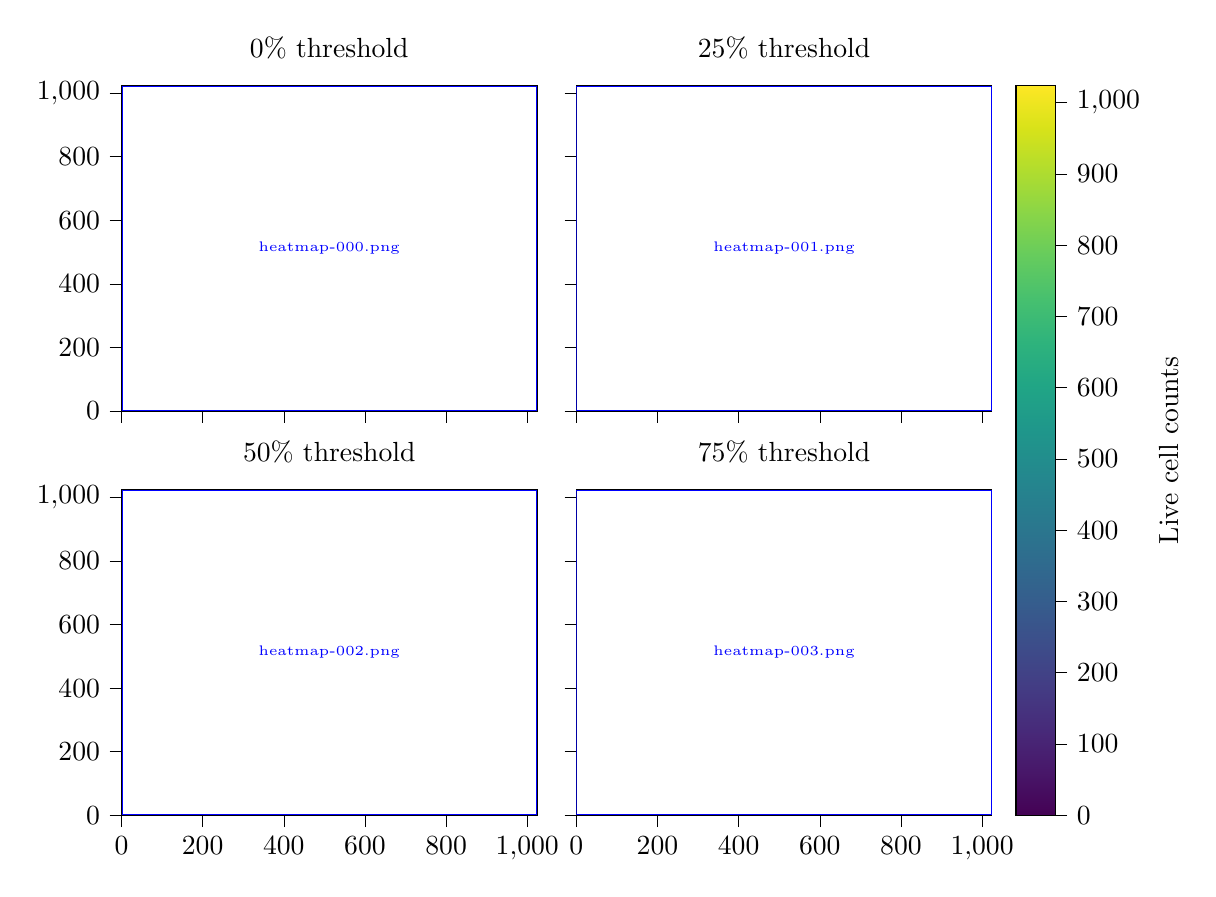
\begin{tikzpicture}

\begin{groupplot}[group style={group size=2 by 2,
    xticklabels at=edge bottom,
    yticklabels at=edge left,
    horizontal sep=0.5cm,
    vertical sep=1cm,
    },
height=0.45\figureheight,
width=0.45\figurewidth,
point meta max=1024,
point meta min=0,
tick align=outside,
tick pos=left,
x grid style={white!69.01960784313725!black},
xmin=0, xmax=1024,
xtick style={color=black},
y grid style={white!69.01960784313725!black},
ymin=0, ymax=1024,
ytick style={color=black}
]
\nextgroupplot[
title={0\% threshold},
]
\addplot graphics [includegraphics cmd=\pgfimage,xmin=0, xmax=1024, ymin=0, ymax=1024] {heatmap-000.png};

\nextgroupplot[
colorbar right,
colormap/viridis,
every colorbar/.append style={height=
  2*\pgfkeysvalueof{/pgfplots/parent axis height}+
  \pgfkeysvalueof{/pgfplots/group/vertical sep}},
colorbar style={ylabel={Live cell counts}, ytick pos=right},
title={25\% threshold},
]
\addplot graphics [includegraphics cmd=\pgfimage,xmin=0, xmax=1024, ymin=0, ymax=1024] {heatmap-001.png};

\nextgroupplot[
title={50\% threshold},
]
\addplot graphics [includegraphics cmd=\pgfimage,xmin=0, xmax=1024, ymin=0, ymax=1024] {heatmap-002.png};

\nextgroupplot[
title={75\% threshold},
]
\addplot graphics [includegraphics cmd=\pgfimage,xmin=0, xmax=1024, ymin=0, ymax=1024] {heatmap-003.png};
\end{groupplot}

\end{tikzpicture}

    \caption{Heatmaps}
    \label{fig:heatmap}
\end{figure}

\begin{figure}
\centering
\setlength\figureheight{5in}
\setlength\figurewidth{6in}
% This file was created by matplotlib2tikz v0.7.3.
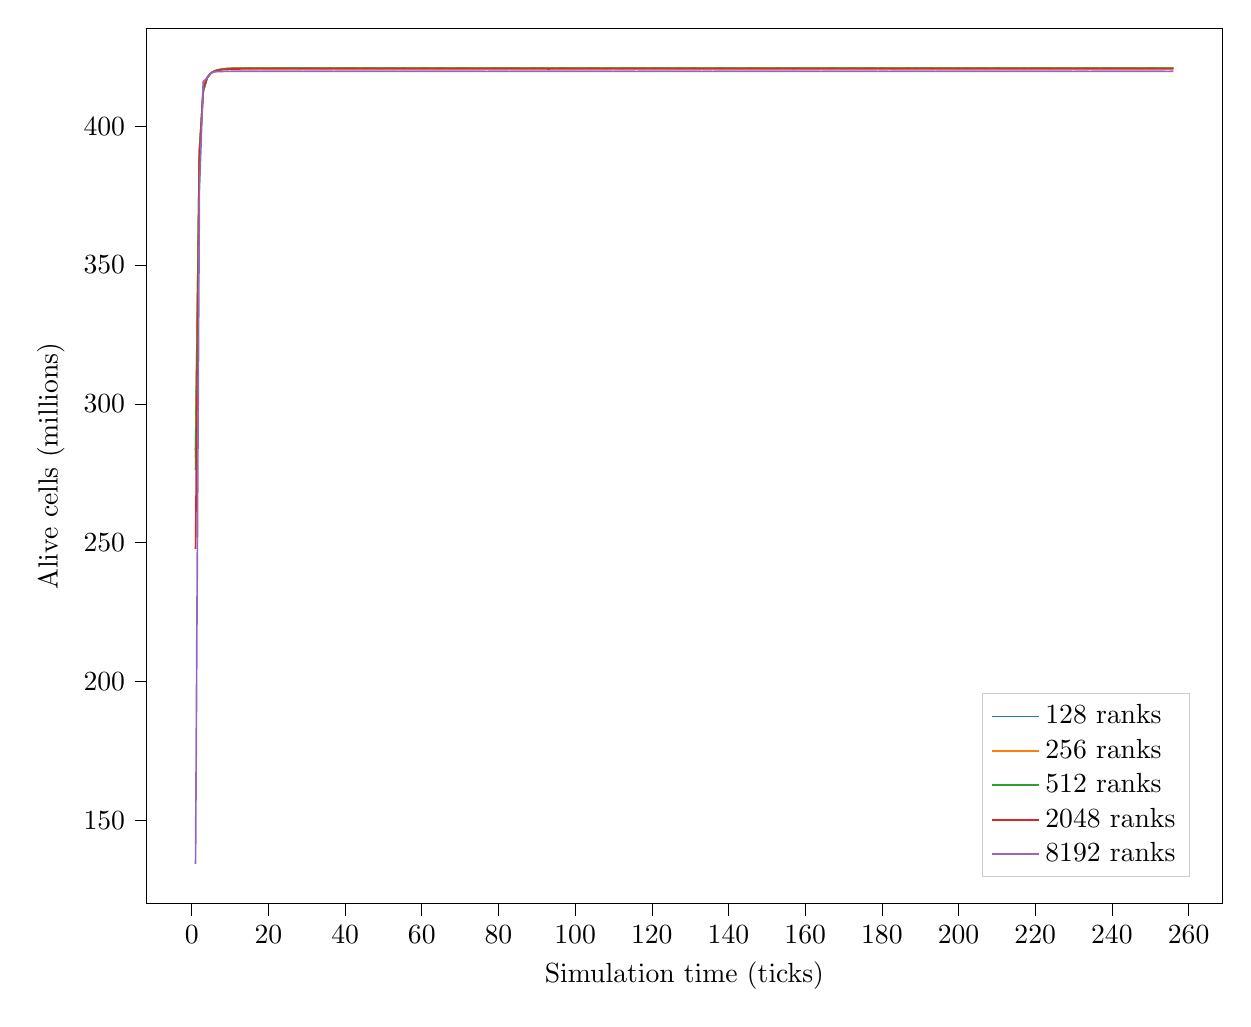
\begin{tikzpicture}

\definecolor{color0}{rgb}{0.12156862745098,0.466666666666667,0.705882352941177}
\definecolor{color1}{rgb}{1,0.498039215686275,0.0549019607843137}
\definecolor{color2}{rgb}{0.172549019607843,0.627450980392157,0.172549019607843}
\definecolor{color3}{rgb}{0.83921568627451,0.152941176470588,0.156862745098039}
\definecolor{color4}{rgb}{0.580392156862745,0.403921568627451,0.741176470588235}

\begin{axis}[
height=\figureheight,
legend cell align={left},
legend style={at={(0.97,0.03)}, anchor=south east, draw=white!80.0!black},
tick align=outside,
tick pos=left,
width=\figurewidth,
x grid style={white!69.01960784313725!black},
xlabel={Simulation time (ticks)},
xmin=-11.75, xmax=268.75,
xtick style={color=black},
y grid style={white!69.01960784313725!black},
ylabel={Alive cells (millions)},
ymin=119.88710325, ymax=435.31348375,
ytick style={color=black}
]
\addplot [semithick, color0]
table {%
1 283.216838
2 390.988255
3 412.449645
4 417.426838
5 419.160083
6 419.910421
7 420.337534
8 420.571253
9 420.756082
10 420.821978
11 420.882584
12 420.895082
13 420.920367
14 420.932479
15 420.960103
16 420.941481
17 420.949151
18 420.93967
19 420.944619
20 420.926932
21 420.956811
22 420.935301
23 420.956181
24 420.952547
25 420.956749
26 420.952246
27 420.951927
28 420.954604
29 420.954897
30 420.964824
31 420.953862
32 420.958733
33 420.95446
34 420.936636
35 420.945653
36 420.97257
37 420.922253
38 420.940959
39 420.957039
40 420.971898
41 420.969826
42 420.950828
43 420.95385
44 420.934061
45 420.956581
46 420.935562
47 420.956073
48 420.951274
49 420.93974
50 420.948155
51 420.975921
52 420.95623
53 420.948853
54 420.932793
55 420.958055
56 420.946431
57 420.947108
58 420.950033
59 420.936984
60 420.952525
61 420.960986
62 420.94744
63 420.936045
64 420.951079
65 420.959347
66 420.945123
67 420.953848
68 420.946785
69 420.95096
70 420.957292
71 420.953671
72 420.960001
73 420.943303
74 420.932114
75 420.964885
76 420.950356
77 420.932298
78 420.945123
79 420.963605
80 420.967487
81 420.95461
82 420.952812
83 420.954367
84 420.959832
85 420.964155
86 420.936179
87 420.941213
88 420.941483
89 420.954908
90 420.948016
91 420.958205
92 420.950247
93 420.934625
94 420.954368
95 420.935984
96 420.960123
97 420.961552
98 420.94474
99 420.956083
100 420.935291
101 420.954838
102 420.93944
103 420.955622
104 420.952662
105 420.954024
106 420.960683
107 420.937917
108 420.952478
109 420.957388
110 420.952112
111 420.939982
112 420.948019
113 420.964311
114 420.949423
115 420.967367
116 420.931755
117 420.948353
118 420.970712
119 420.964592
120 420.953977
121 420.955146
122 420.95589
123 420.939074
124 420.960622
125 420.945638
126 420.924845
127 420.963172
128 420.949265
129 420.937254
130 420.950341
131 420.969325
132 420.941958
133 420.938211
134 420.949256
135 420.946603
136 420.936897
137 420.945979
138 420.964415
139 420.938616
140 420.92799
141 420.962685
142 420.94529
143 420.929165
144 420.941575
145 420.954292
146 420.963677
147 420.955103
148 420.964962
149 420.950125
150 420.941156
151 420.948069
152 420.949229
153 420.960345
154 420.934294
155 420.96282
156 420.952989
157 420.953076
158 420.965333
159 420.943462
160 420.942538
161 420.948456
162 420.949015
163 420.941279
164 420.940582
165 420.944632
166 420.947651
167 420.963254
168 420.949459
169 420.943229
170 420.93866
171 420.951179
172 420.951009
173 420.960617
174 420.942034
175 420.943089
176 420.964969
177 420.951168
178 420.956552
179 420.931612
180 420.966287
181 420.943496
182 420.936111
183 420.948343
184 420.945169
185 420.938729
186 420.945048
187 420.955281
188 420.947854
189 420.953715
190 420.944904
191 420.966783
192 420.945478
193 420.958945
194 420.943978
195 420.953435
196 420.949452
197 420.960518
198 420.951503
199 420.936677
200 420.955375
201 420.932492
202 420.966356
203 420.940413
204 420.941479
205 420.962066
206 420.958018
207 420.956373
208 420.940419
209 420.938549
210 420.968108
211 420.947616
212 420.940356
213 420.949218
214 420.945802
215 420.95311
216 420.940955
217 420.959543
218 420.944245
219 420.950957
220 420.951259
221 420.947671
222 420.965018
223 420.949735
224 420.955372
225 420.940359
226 420.955306
227 420.946768
228 420.947657
229 420.947106
230 420.942647
231 420.941537
232 420.936912
233 420.959166
234 420.961169
235 420.942908
236 420.95926
237 420.92894
238 420.9569
239 420.952875
240 420.951665
241 420.968769
242 420.961851
243 420.958894
244 420.944988
245 420.947386
246 420.951717
247 420.944138
248 420.945794
249 420.946261
250 420.951364
251 420.961286
252 420.939398
253 420.946977
254 420.932573
255 420.937136
256 420.954669
};
\addlegendentry{128 ranks}
\addplot [semithick, color1]
table {%
1 280.851673
2 390.80109
3 412.525556
4 417.423935
5 419.161913
6 419.908694
7 420.331025
8 420.561353
9 420.741404
10 420.807277
11 420.868713
12 420.877839
13 420.897685
14 420.920413
15 420.935992
16 420.925
17 420.932284
18 420.925858
19 420.928283
20 420.903895
21 420.938013
22 420.916795
23 420.942357
24 420.934867
25 420.930189
26 420.93041
27 420.934135
28 420.934995
29 420.93667
30 420.946591
31 420.94015
32 420.941928
33 420.936281
34 420.920888
35 420.934516
36 420.950904
37 420.913838
38 420.928021
39 420.935632
40 420.949591
41 420.945258
42 420.93238
43 420.937325
44 420.921983
45 420.934493
46 420.917554
47 420.928392
48 420.93386
49 420.931674
50 420.915586
51 420.946504
52 420.943852
53 420.940917
54 420.915411
55 420.938349
56 420.930405
57 420.93715
58 420.940867
59 420.923451
60 420.938005
61 420.939082
62 420.932856
63 420.924759
64 420.932117
65 420.944035
66 420.92542
67 420.935245
68 420.928516
69 420.935805
70 420.931003
71 420.938267
72 420.941967
73 420.906783
74 420.924291
75 420.948552
76 420.934765
77 420.911138
78 420.92819
79 420.929032
80 420.951444
81 420.94475
82 420.943856
83 420.928761
84 420.945302
85 420.95051
86 420.920848
87 420.94352
88 420.924766
89 420.943312
90 420.91947
91 420.935747
92 420.934997
93 420.912921
94 420.937182
95 420.933198
96 420.947744
97 420.936024
98 420.911669
99 420.926679
100 420.922446
101 420.923519
102 420.934293
103 420.921252
104 420.9426
105 420.935128
106 420.936442
107 420.932304
108 420.943377
109 420.943182
110 420.920106
111 420.940461
112 420.915821
113 420.932061
114 420.928896
115 420.929876
116 420.916745
117 420.946683
118 420.940736
119 420.959074
120 420.946265
121 420.932637
122 420.934146
123 420.925927
124 420.94078
125 420.942325
126 420.926454
127 420.923437
128 420.930545
129 420.924613
130 420.938039
131 420.944533
132 420.934571
133 420.922263
134 420.932754
135 420.930268
136 420.918788
137 420.943572
138 420.934206
139 420.91893
140 420.928232
141 420.925024
142 420.914023
143 420.925951
144 420.949888
145 420.948425
146 420.941247
147 420.927829
148 420.948152
149 420.928138
150 420.933749
151 420.913362
152 420.954557
153 420.934832
154 420.939693
155 420.939071
156 420.934425
157 420.942678
158 420.938091
159 420.920666
160 420.932382
161 420.936367
162 420.929376
163 420.928064
164 420.919104
165 420.934379
166 420.938171
167 420.926859
168 420.931083
169 420.925242
170 420.936835
171 420.931966
172 420.95399
173 420.935104
174 420.927646
175 420.923356
176 420.947461
177 420.92495
178 420.933241
179 420.926088
180 420.950546
181 420.925985
182 420.923241
183 420.907447
184 420.917612
185 420.919748
186 420.936178
187 420.93556
188 420.931198
189 420.9275
190 420.939053
191 420.948179
192 420.944718
193 420.923762
194 420.926632
195 420.929453
196 420.92901
197 420.942045
198 420.945123
199 420.916982
200 420.930665
201 420.915527
202 420.952324
203 420.941436
204 420.928106
205 420.946735
206 420.915895
207 420.952492
208 420.926165
209 420.941987
210 420.922339
211 420.933766
212 420.932239
213 420.927832
214 420.9452
215 420.929623
216 420.93111
217 420.942909
218 420.925845
219 420.925501
220 420.930152
221 420.92853
222 420.945985
223 420.926902
224 420.940018
225 420.926437
226 420.928405
227 420.955024
228 420.930854
229 420.949647
230 420.905736
231 420.926066
232 420.926806
233 420.945978
234 420.913728
235 420.92734
236 420.939557
237 420.940688
238 420.942824
239 420.934248
240 420.933336
241 420.92715
242 420.936178
243 420.94411
244 420.930789
245 420.944483
246 420.931633
247 420.90902
248 420.918216
249 420.934715
250 420.945374
251 420.946655
252 420.92963
253 420.928597
254 420.924692
255 420.934196
256 420.936072
};
\addlegendentry{256 ranks}
\addplot [semithick, color2]
table {%
1 276.120093
2 390.423456
3 412.688411
4 417.418248
5 419.159249
6 419.907384
7 420.313677
8 420.535269
9 420.703985
10 420.767176
11 420.840748
12 420.848841
13 420.87041
14 420.879456
15 420.899073
16 420.887046
17 420.894664
18 420.882752
19 420.897673
20 420.876235
21 420.895078
22 420.89448
23 420.909475
24 420.907007
25 420.882649
26 420.915733
27 420.895483
28 420.895418
29 420.896638
30 420.894084
31 420.908004
32 420.921424
33 420.903734
34 420.892383
35 420.900464
36 420.918022
37 420.867358
38 420.899927
39 420.88436
40 420.900506
41 420.911823
42 420.875967
43 420.890947
44 420.881053
45 420.89191
46 420.896622
47 420.882137
48 420.894497
49 420.89546
50 420.885151
51 420.907493
52 420.903133
53 420.896837
54 420.884692
55 420.901163
56 420.894716
57 420.903321
58 420.906787
59 420.891906
60 420.891491
61 420.908208
62 420.892823
63 420.87422
64 420.891686
65 420.897687
66 420.898778
67 420.90227
68 420.897771
69 420.89938
70 420.890719
71 420.904098
72 420.914404
73 420.890378
74 420.883145
75 420.893218
76 420.898629
77 420.87375
78 420.886538
79 420.902045
80 420.925596
81 420.899277
82 420.89941
83 420.884612
84 420.90998
85 420.906744
86 420.900538
87 420.886792
88 420.903095
89 420.899141
90 420.883563
91 420.902781
92 420.904299
93 420.885072
94 420.900301
95 420.887817
96 420.895884
97 420.901769
98 420.881936
99 420.895545
100 420.895635
101 420.891041
102 420.891576
103 420.873965
104 420.90921
105 420.888736
106 420.902325
107 420.89394
108 420.894289
109 420.893043
110 420.898057
111 420.885143
112 420.888268
113 420.876963
114 420.883718
115 420.893679
116 420.891414
117 420.905874
118 420.908571
119 420.924083
120 420.897471
121 420.888434
122 420.897047
123 420.875288
124 420.875902
125 420.894259
126 420.885439
127 420.88201
128 420.880062
129 420.890075
130 420.902456
131 420.909132
132 420.892596
133 420.894818
134 420.896309
135 420.903122
136 420.910189
137 420.903843
138 420.911228
139 420.888825
140 420.882314
141 420.880347
142 420.897069
143 420.896468
144 420.875675
145 420.884114
146 420.905838
147 420.890755
148 420.920438
149 420.888682
150 420.897852
151 420.890958
152 420.905037
153 420.888557
154 420.900346
155 420.921735
156 420.888131
157 420.881445
158 420.884397
159 420.900214
160 420.903982
161 420.88102
162 420.889557
163 420.895132
164 420.876469
165 420.903247
166 420.896874
167 420.922836
168 420.899287
169 420.894598
170 420.899559
171 420.902646
172 420.90294
173 420.903792
174 420.895992
175 420.898031
176 420.902194
177 420.894169
178 420.903678
179 420.900531
180 420.9001
181 420.883269
182 420.883039
183 420.883525
184 420.883369
185 420.882794
186 420.904332
187 420.910658
188 420.88823
189 420.877387
190 420.905864
191 420.905377
192 420.90161
193 420.911148
194 420.890113
195 420.885975
196 420.895129
197 420.908598
198 420.912304
199 420.879626
200 420.900005
201 420.893552
202 420.909126
203 420.895769
204 420.88611
205 420.9046
206 420.891818
207 420.901302
208 420.904348
209 420.881597
210 420.909857
211 420.896232
212 420.893881
213 420.900425
214 420.886073
215 420.878027
216 420.899201
217 420.907786
218 420.889714
219 420.895129
220 420.897774
221 420.892803
222 420.897421
223 420.878084
224 420.901554
225 420.886285
226 420.905093
227 420.887663
228 420.915664
229 420.898862
230 420.883892
231 420.898462
232 420.88865
233 420.919552
234 420.888207
235 420.887636
236 420.901179
237 420.901994
238 420.898798
239 420.894464
240 420.8934
241 420.893643
242 420.916307
243 420.883057
244 420.904276
245 420.901109
246 420.891882
247 420.89276
248 420.903974
249 420.886861
250 420.904619
251 420.907165
252 420.886322
253 420.893855
254 420.889959
255 420.885735
256 420.893741
};
\addlegendentry{512 ranks}
\addplot [semithick, color3]
table {%
1 247.742614
2 388.182608
3 413.658537
4 417.388003
5 419.152536
6 419.861609
7 420.215428
8 420.378934
9 420.524258
10 420.580289
11 420.626539
12 420.631465
13 420.655717
14 420.682815
15 420.661942
16 420.660858
17 420.680891
18 420.678918
19 420.681725
20 420.651946
21 420.66601
22 420.683661
23 420.679866
24 420.676346
25 420.678095
26 420.679744
27 420.680714
28 420.669894
29 420.672365
30 420.678893
31 420.683576
32 420.693731
33 420.668754
34 420.656002
35 420.669104
36 420.698456
37 420.659956
38 420.691811
39 420.666001
40 420.693492
41 420.679096
42 420.666908
43 420.65584
44 420.662071
45 420.684873
46 420.683897
47 420.674484
48 420.675781
49 420.670924
50 420.663094
51 420.656443
52 420.675599
53 420.675043
54 420.664277
55 420.693687
56 420.675142
57 420.668
58 420.660803
59 420.65962
60 420.687176
61 420.680597
62 420.668115
63 420.66875
64 420.678123
65 420.685407
66 420.686368
67 420.668261
68 420.659342
69 420.68198
70 420.688333
71 420.678184
72 420.691854
73 420.666305
74 420.663976
75 420.68533
76 420.667877
77 420.649767
78 420.684543
79 420.688314
80 420.692363
81 420.666808
82 420.683818
83 420.680204
84 420.698742
85 420.702945
86 420.657888
87 420.665135
88 420.668313
89 420.69567
90 420.667448
91 420.681984
92 420.687008
93 420.634562
94 420.674662
95 420.675286
96 420.683218
97 420.705723
98 420.67377
99 420.675563
100 420.682006
101 420.66722
102 420.682249
103 420.653938
104 420.684068
105 420.687594
106 420.668616
107 420.670593
108 420.676551
109 420.679426
110 420.670119
111 420.665883
112 420.670248
113 420.675416
114 420.673709
115 420.688667
116 420.660346
117 420.684885
118 420.68232
119 420.684847
120 420.675125
121 420.647465
122 420.673828
123 420.681687
124 420.671388
125 420.672234
126 420.662397
127 420.676134
128 420.669868
129 420.66687
130 420.689378
131 420.684017
132 420.678126
133 420.664017
134 420.674163
135 420.661283
136 420.667958
137 420.689603
138 420.685555
139 420.664455
140 420.663016
141 420.675298
142 420.663328
143 420.669526
144 420.680625
145 420.679773
146 420.693994
147 420.664611
148 420.682173
149 420.671808
150 420.684197
151 420.671008
152 420.682405
153 420.694586
154 420.664218
155 420.684614
156 420.675751
157 420.646836
158 420.694696
159 420.664821
160 420.664007
161 420.669433
162 420.67468
163 420.677262
164 420.654445
165 420.678061
166 420.674533
167 420.685336
168 420.666762
169 420.665436
170 420.661884
171 420.670172
172 420.65964
173 420.662548
174 420.666489
175 420.667054
176 420.702583
177 420.678682
178 420.663679
179 420.678837
180 420.68954
181 420.694001
182 420.652878
183 420.665246
184 420.663911
185 420.662801
186 420.680643
187 420.701623
188 420.670508
189 420.65968
190 420.673948
191 420.669515
192 420.687812
193 420.688847
194 420.665496
195 420.669391
196 420.669888
197 420.677925
198 420.687492
199 420.666685
200 420.694056
201 420.652663
202 420.704837
203 420.683883
204 420.670187
205 420.686648
206 420.667703
207 420.684395
208 420.671055
209 420.673397
210 420.662445
211 420.667917
212 420.67282
213 420.671949
214 420.686295
215 420.675187
216 420.659187
217 420.68024
218 420.650576
219 420.682765
220 420.673816
221 420.692715
222 420.690718
223 420.665476
224 420.682664
225 420.666075
226 420.673959
227 420.68925
228 420.682996
229 420.682929
230 420.672343
231 420.693951
232 420.664826
233 420.681975
234 420.673776
235 420.68129
236 420.674122
237 420.670422
238 420.688233
239 420.68196
240 420.673412
241 420.677284
242 420.67662
243 420.671928
244 420.692202
245 420.682253
246 420.691927
247 420.667956
248 420.673305
249 420.682428
250 420.697384
251 420.666998
252 420.672699
253 420.677246
254 420.679195
255 420.659847
256 420.682621
};
\addlegendentry{2048 ranks}
\addplot [semithick, color4]
table {%
1 134.224666
2 376.890357
3 416.099023
4 417.328279
5 419.202607
6 419.621089
7 419.701104
8 419.731264
9 419.788528
10 419.772646
11 419.811727
12 419.798714
13 419.804117
14 419.792797
15 419.820599
16 419.795741
17 419.793091
18 419.777688
19 419.796679
20 419.777789
21 419.814399
22 419.821416
23 419.79436
24 419.8238
25 419.781903
26 419.816415
27 419.777965
28 419.81726
29 419.771479
30 419.810353
31 419.777929
32 419.822108
33 419.785166
34 419.785245
35 419.80476
36 419.813265
37 419.771257
38 419.811691
39 419.791194
40 419.82155
41 419.789884
42 419.784681
43 419.806624
44 419.805516
45 419.803327
46 419.799258
47 419.798907
48 419.78578
49 419.796434
50 419.782
51 419.801105
52 419.792792
53 419.788039
54 419.776576
55 419.821685
56 419.794036
57 419.796277
58 419.786856
59 419.813585
60 419.795111
61 419.805243
62 419.790696
63 419.786739
64 419.794273
65 419.809657
66 419.79632
67 419.788408
68 419.79767
69 419.817815
70 419.806157
71 419.793127
72 419.805689
73 419.784503
74 419.789608
75 419.817135
76 419.792796
77 419.766067
78 419.823328
79 419.805314
80 419.800207
81 419.817836
82 419.794163
83 419.772279
84 419.823531
85 419.819904
86 419.789399
87 419.804338
88 419.787604
89 419.811628
90 419.815023
91 419.803517
92 419.809049
93 419.785502
94 419.790421
95 419.788284
96 419.809386
97 419.799908
98 419.787269
99 419.801578
100 419.80866
101 419.807116
102 419.806082
103 419.784268
104 419.817172
105 419.787088
106 419.794453
107 419.794943
108 419.792902
109 419.792495
110 419.77496
111 419.797633
112 419.787759
113 419.78403
114 419.807551
115 419.802128
116 419.763917
117 419.803753
118 419.807277
119 419.814755
120 419.787504
121 419.786219
122 419.802469
123 419.798271
124 419.8079
125 419.811767
126 419.782763
127 419.78871
128 419.797311
129 419.804598
130 419.81228
131 419.804627
132 419.799957
133 419.776018
134 419.787973
135 419.791749
136 419.770625
137 419.819497
138 419.811045
139 419.795502
140 419.778509
141 419.807728
142 419.78372
143 419.781711
144 419.782776
145 419.805506
146 419.802706
147 419.794106
148 419.804712
149 419.788197
150 419.792474
151 419.806227
152 419.807932
153 419.812957
154 419.791171
155 419.807477
156 419.783838
157 419.788255
158 419.787786
159 419.784505
160 419.794053
161 419.797215
162 419.801032
163 419.803415
164 419.774007
165 419.794444
166 419.825158
167 419.803998
168 419.791758
169 419.791955
170 419.788565
171 419.819825
172 419.810734
173 419.80013
174 419.800936
175 419.789622
176 419.802741
177 419.805787
178 419.802309
179 419.769756
180 419.827981
181 419.790682
182 419.774694
183 419.811595
184 419.784564
185 419.783065
186 419.8042
187 419.818072
188 419.803501
189 419.792724
190 419.786626
191 419.801992
192 419.801384
193 419.787883
194 419.777045
195 419.804653
196 419.782877
197 419.798457
198 419.803263
199 419.784996
200 419.791377
201 419.786789
202 419.794523
203 419.803844
204 419.795178
205 419.800725
206 419.783444
207 419.817524
208 419.783315
209 419.794325
210 419.811581
211 419.811416
212 419.795927
213 419.799932
214 419.805133
215 419.780637
216 419.793999
217 419.810869
218 419.786373
219 419.793163
220 419.801302
221 419.80095
222 419.816244
223 419.793286
224 419.807447
225 419.79204
226 419.781499
227 419.800448
228 419.800749
229 419.796504
230 419.768703
231 419.803387
232 419.795374
233 419.797837
234 419.776994
235 419.780927
236 419.806384
237 419.803978
238 419.800778
239 419.799995
240 419.801718
241 419.807015
242 419.795884
243 419.792256
244 419.788552
245 419.812832
246 419.801212
247 419.796283
248 419.780535
249 419.807385
250 419.79957
251 419.81777
252 419.787931
253 419.791061
254 419.778106
255 419.775762
256 419.80159
};
\addlegendentry{8192 ranks}
\end{axis}

\end{tikzpicture}
\caption{The number of alive cells in given ticks with threshold of 25\%.}
\label{fig:alive-cells}
\end{figure}
\end{document}
